% Compile with XeLaTeX or Tectonic. Main body: four pages; appendix is separate.
\documentclass[10pt,a4paper]{article}
\usepackage[top=14mm,bottom=15mm,left=17mm,right=17mm]{geometry}
\usepackage{fontspec,xeCJK}
\IfFontExistsTF{Times New Roman}{\setmainfont{Times New Roman}}{\setmainfont{Latin Modern Roman}}
\IfFontExistsTF{Songti SC}{
  \setCJKmainfont{Songti SC}[AutoFakeBold=2]
  \setCJKsansfont{Heiti SC}
}{
  \setCJKmainfont{FandolSong-Regular.otf}[BoldFont=FandolSong-Bold.otf]
  \setCJKsansfont{FandolHei-Regular.otf}
}
\IfFontExistsTF{Menlo}{\setmonofont{Menlo}[Scale=0.87]}{\setmonofont{Latin Modern Mono}[Scale=0.9]}
\usepackage{amsmath,amssymb,booktabs,array,longtable,graphicx,xcolor,enumitem}
\usepackage{unicode-math}
\setmathfont{latinmodern-math.otf}
\usepackage[font=small,labelfont=bf,skip=3pt]{caption}
\usepackage[colorlinks=true,linkcolor=blue!45!black,urlcolor=blue!45!black]{hyperref}
\hypersetup{pdftitle={OpenMP IVF-Flat 向量检索实验报告},pdfauthor={刘师妤}}
\setlength{\parindent}{2em}
\setlength{\parskip}{2.5pt}
\setlength{\tabcolsep}{4.2pt}
\renewcommand{\arraystretch}{1.12}
\setlength{\abovedisplayskip}{5pt}
\setlength{\belowdisplayskip}{5pt}
\setlength{\textfloatsep}{6pt}
\setlength{\intextsep}{6pt}
\setlength{\emergencystretch}{1.5em}
\setlist{nosep,leftmargin=1.7em}
\renewcommand{\figurename}{图}
\renewcommand{\tablename}{表}
\makeatletter
\renewcommand\section{\@startsection{section}{1}{0pt}{7pt}{4pt}{\large\bfseries}}
\renewcommand\subsection{\@startsection{subsection}{2}{0pt}{5pt}{2pt}{\normalsize\bfseries}}
\makeatother
\newcommand{\code}[1]{\texttt{\detokenize{#1}}}
\newcommand{\lead}[1]{\noindent\textbf{#1}\quad}
\newcommand{\smalltable}{\fontsize{9}{11}\selectfont}
\newcommand{\runid}[1]{\texttt{run\_#1}}
\graphicspath{{figures/}{../figures/}}
\raggedbottom
\AtBeginDocument{\fontsize{10.3}{14.2}\selectfont}

\begin{document}
\begin{center}
{\LARGE\bfseries OpenMP IVF-Flat 向量检索实验报告}\par\vspace{3pt}
刘师妤\quad 2024201568\qquad 实验日期：2026-11-05
\end{center}
\vspace{-5pt}

\section{检索过程与并行方案}
IVF-Flat 先比较查询与 $L$ 个中心，选取最近的 $n_{\rm probe}$ 个列表，再计算其中全部候选的平方欧氏距离，按 $(\mathrm{distance},\mathrm{id})$ 选出 Top-$k$。
设选中列表为 $\mathcal P(q)$、列表长度为 $|I_l|$，则
\[
 D(q,x)=\sum_{j=0}^{d-1}(\mathrm{double}(q_j)-\mathrm{double}(x_j))^2,
 \qquad C(q)=\sum_{l\in\mathcal P(q)}|I_l|.
\]
两种并行方向由题目规定。本实现围绕任务粒度、私有结果与同步位置作选择，使各版本计算相同的中心与候选集合，便于比较并行组织本身的收益。

\subsection{omp1：连续静态分配查询}
一次 batch 调用进入一个团队，以 \code{omp for schedule(static)} 分配查询；每个查询独立完成中心选择、候选扫描和 Top-$k$。索引只读，查询 $q$ 仅写输出区间 $[qk,(q+1)k)$，没有共享堆。
选择 static 是为了建立调度成本低、工作归属明确的基线，并与 std 的连续区间分配对应；其代价是按查询数均分，未考虑 $C(q)$。当 batch=1 时只有一个循环迭代，增加线程不能拆开该查询。dynamic 可作为后续调度对照，本轮未测其性能，因而不将 static 称为最优调度。

\subsection{omp2：一个团队中的查询父任务与候选子任务}
\code{single} 为 batch 内各查询创建父 task。每个父任务调用公共标量中心选择，沿各选中列表的连续位置区间切块，再生成距离计算子 task。不同查询的中心选择可由不同父任务同时执行；单查询内部，候选块在同一团队中调度。若在 \code{single} 中串行完成所有查询的中心选择，会把跨查询并行机会留在主线程上，因此这里将中心选择放入父任务。

\begin{center}
\small
\begin{tabular}{p{.25\linewidth}p{.65\linewidth}}
\toprule
阶段 & 数据所有权与完成条件 \\
\midrule
选择、切块与分配 & 父任务持有块描述、$B(q)k$ 个局部结果槽及逐块异常记录。\\
子任务扫描 & \code{firstprivate} 保存块编号、查询指针和 $k$；每块用自己的 TopK，只写对应结果切片。\\
等待、合并与释放 & \code{taskgroup} 完成后才读局部输出、合并和销毁父任务数组；退出团队前完成全部查询。\\
\bottomrule
\end{tabular}
\end{center}

本实现逐列表切块，不把短列表拼接。每块最多 $g=\mathrm{grain}$ 个候选，块数为
\[
B(q)=\sum_{l\in\mathcal P(q)}\left\lceil\frac{|I_l|}{g}\right\rceil,
\qquad |I_l|=0\text{ 时贡献为 }0.
\]
这使长列表也能拆分，选中列表的区间无重叠、无遗漏，每个候选恰好计算一次。当前对全部非空块生成任务，未加入未经实验校准的小任务阈值。

\lead{局部 Top-$k$ 足够的原因。}
若候选 $x$ 被本块 Top-$k$ 排除，本块至少有 $k$ 项在统一全序下排在 $x$ 前；这些项在全局仍优于 $x$，所以 $x$ 不可能进入全局 Top-$k$。因此只需合并局部结果的并集。
局部数组为 $O(Bk)$，任务数为 $O(B)$，以大小为 $k$ 的堆扫描至多 $Bk$ 个局部结果，合并成本为 $O(Bk\log k)$。相比每候选更新共享堆，这一组织把频繁竞争改为任务私有计算和一次合并；代码没有逐候选 critical，也没有嵌套团队。

\lead{SIMD 与 std 对照。}
SIMD 只替换候选距离：double 差值、平方和归约使用 \code{omp simd reduction(+:sum)}，归约结束后更新 Top-$k$，避免将堆依赖混入维度循环。中心选择保留公共标量函数，确保选择相同列表。std 则连续均分查询，每批实际有 $m$ 个查询时创建 $\min(p,m)$ 个线程，完成后 join；创建、绑定和回收均在计时内。

\newpage
\section{实验条件、正确性与 A：线程扩展}
\lead{资源与参数。}
完整 SIFT1M：$N=10^6,d=128,L=4096,Q=128,k=10$；默认 $n_{\rm probe}=8,g=1024$。Linux 5.15.0-60、GCC 11.4.0、libgomp，\code{-O3 -std=c++17 -fopenmp -pthread}，无 fast-math 或 march=native。机器报告 Xeon Gold 5218 @ 2.30GHz、49 GiB 内存、CPU 0--31；具有 hypervisor 标记。$P=32$ 是客户机可见预算，宿主物理核心及 SMT 分配未知。
各版本先由 taskset 限定同一 CPU 集合，串行及调用线程绑定 CPU 0，std 槽 $t$ 绑定 CPU $t$；OpenMP 显式设置 \code{OMP_PLACES={0},...,{31}}、\code{OMP_PROC_BIND=close}、\code{OMP_DYNAMIC=FALSE}、\code{OMP_WAIT_POLICY=PASSIVE}。独立统计的 10,294 个有效端点与绑定一致；该采样覆盖工作记录端点，而非完整迁移轨迹。

\lead{计时与验证。}
每配置预热一次、正式重复十次，使用 steady\_clock。$T$ 为全部同步 batch 调用的墙钟时间之和，包含中心选择、分块、分配、距离、堆、合并、线程管理和同步；加载、参考生成、预热、检查与输出在外。每次重新计算并逐项检查输出。统计另跑，通过编译期模板将计数与阶段时钟排除在普通 bench 实例外。报告 $\mathrm{QPS}=Q/T$、$S=T_{\rm IVF,serial}/T_p$、$E=S/p$。
公共测试、2,905 个学生实现配置、48 个统计配置和 CLI 测试通过；正式 40 配置共 400 次重复全部通过，另有 40 次独立诊断。16,910 个 batch 样本与每轮总时间相符，五个数据及 13 个实验源码哈希匹配。边界测试覆盖空列表、少于 $k$、等距、$k=1$ 和全列表扫描；此前真实数据 pilot 的 24 组检查包括全库参考。ID 一致，距离容差为 $10^{-10}$，不足项填 $(-1,+\infty)$。

\begin{center}
\smalltable
\begin{tabular}{rrrrrrr}
\toprule
$p$ & \multicolumn{2}{c}{batch=1：$T$ (ms)} & \multicolumn{4}{c}{batch=128：$T$ (ms)、$S$ / $E$}\\
 & omp1 & omp2 & omp1 $T$ & omp1 $S/E$ & omp2 $T$ & omp2 $S/E$\\
\midrule
1 &116.067&131.452&114.062&1.00 / 99.9\%&125.224&0.91 / 91.0\%\\
2 &115.640&124.045&60.874&1.87 / 93.5\%&67.951&1.68 / 83.8\%\\
4 &128.920&206.308&44.617&2.55 / 63.8\%&34.267&3.32 / 83.1\%\\
8 &150.250&230.304&27.077&4.21 / 52.6\%&19.541&5.83 / 72.9\%\\
16&198.063&311.057&13.494&8.44 / 52.8\%&11.961&9.52 / 59.5\%\\
32&324.547&380.034&9.653&11.80 / 36.9\%&7.946&14.33 / 44.8\%\\
\bottomrule
\end{tabular}
\end{center}
\noindent\small 全部为标量距离，中位时间覆盖 128 个查询。两个 batch 的串行基线分别为 113.690、113.895 ms；大 batch 固定 $4P=128$，不随 $p$ 变化。\normalsize
\begin{center}
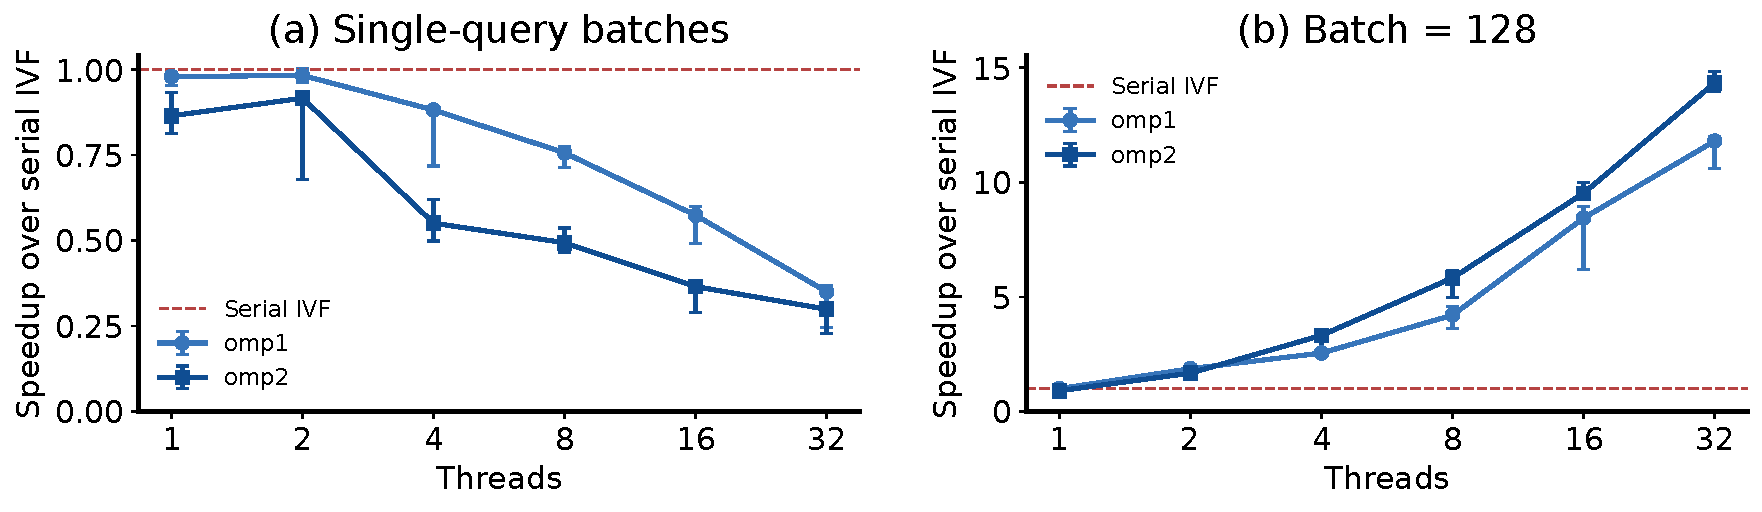
\includegraphics[width=.94\linewidth]{scaling.pdf}
\captionof{figure}{中位加速比；误差线用并行时间 min/max 换算，串行分子固定为中位数。}
\end{center}
\lead{批量收益与单查询负优化。}
batch=128、$p=32$ 时 omp1 的 min/med/max 为 9.492/9.653/10.740 ms，omp2 为 7.682/7.946/8.160 ms，分别为 13,261、16,108 QPS。omp2 比 omp1 快 1.21 倍。
batch=1 时 omp1 只有一个候选工作线程，omp2 最多九个、平均每查询仅 8.05 个子任务；单查询中心选择仍串行，每批团队同步与 PASSIVE 唤醒成本难以分摊。三者单查询延迟 p50/p95 分别为 serial 0.854/1.154、omp1 2.418/3.389、omp2 2.956/3.382 ms（$p=32$）。该对照支持少查询时避免盲目增加线程；同步等因素的各自占比尚未隔离。

\newpage
\section{B/C：工作分配、任务粒度与线程对照}
\subsection{B：同一查询池排序，检验按数量均分是否合理}
列表长度中位数 227、最大 1,257；$C(q)$ 中位数 2,122、最大 5,395，128 个查询共 296,624 个候选。原始、升序、降序使用同一查询池，同步重排 ground truth；固定 $p=32$、batch=128、标量距离和 $g=1024$，候选集合与 Recall 不变。独立统计以 $W_t$ 表示线程槽的候选计算数，包含零计数槽，核对 $\sum_tW_t=296624$。
\begin{center}
\smalltable
\begin{tabular}{lrrrrrr}
\toprule
 &\multicolumn{3}{c}{中位时间 (ms)}&\multicolumn{3}{c}{$\max W_t/\operatorname{mean}W_t$}\\
策略&原始&升序&降序&原始&升序&降序\\
\midrule
omp1&9.653&11.493&10.125&1.392&2.223&2.223\\
omp2&7.946&8.084&8.038&1.524&1.461&1.839\\
\bottomrule
\end{tabular}
\end{center}
omp1 静态连续分配给每线程四个查询。排序将轻查询聚到一端、重查询聚到另一端，使平均查询数相同但候选数更不均；升序慢 19.1\%，降序慢 4.9\%。这是固定查询集合的排序消融，支持 static 对工作量顺序敏感的解释。两种排序的候选失衡相同而时间不同，也说明 $W_t$ 只刻画部分工作：中心选择、调度与访问顺序还会影响时间，局部性贡献需要进一步计数验证。
omp2 的父任务和候选块由同一团队执行，各排序中位时间变化不超过 1.8\%；候选分配较灵活，但一次独立诊断不能代表十轮中的每轮工作分配。原始顺序下 omp2 的候选失衡值甚至高于 omp1，而耗时更少，因此不能仅按这一指标排列策略优劣。

\subsection{C：grain 同时控制任务数、缓冲区与合并工作}
固定 omp2、$p=32$、batch=128、$n_{\rm probe}=8$；每次除子任务外还有 128 个查询父任务。下表“数组”为单查询局部结果、描述及异常数组的最大实际容量字节数，未包括运行时 task 对象、中心临时数组、分配器和其他查询；活动子任务堆另有上界字段，故该列不是进程峰值。
\begin{center}
\smalltable
\begin{tabular}{rrrrrr}
\toprule
grain&子任务&$T_{\min}/T_{\rm med}/T_{\max}$ (ms)&数组 (B)&合并区间和 (ms)&taskgroup 区间和 (ms)\\
\midrule
64&5,147&9.724 / 10.377 / 10.664&16,832&0.980&173.955\\
256&1,607&7.734 / 7.793 / 8.293&4,880&0.567&134.786\\
1024&1,030&7.682 / 7.946 / 8.160&1,768&0.445&121.019\\
4096&1,024&11.364 / 37.877 / 75.667&1,472&0.455&130.954\\
\bottomrule
\end{tabular}
\end{center}
grain=64 比 1024 产生约五倍子任务，合并区间之和增至 2.20 倍，中位时间增加 30.6\%，支持过细任务增加管理成本。由于各查询会并发，合并及 taskgroup 列是\textbf{独立诊断中各查询墙钟区间之和}，不能相加当批完成时间，也不能除以正式 $T$ 当阶段占比；taskgroup 区间还包含任务执行与等待。

grain=256 的中位数比 1024 少 1.9\%，十次范围重叠，1024 继续作为统一对照参数；它是预先固定的基准，不是事后筛出的最优值。grain=4096 的波动范围很大，且只比 1024 少六个子任务。原因在于逐列表切块：$g\ge1257$ 时，每个选中的非空列表均为一个块，$128\times8=1024$；$g=1024$ 只额外切开少量长列表。因此无法把异常直接归因于“任务数骤降”。需交替复测并记录资源状态后再作因果判断，原始异常完整保留。

\subsection{std 对照与实现代价}
同一大 batch、32 线程、相同距离与绑定下，std 的 min/med/max 为 10.470/10.875/12.158 ms，QPS=11,770、$S=10.47$；omp1 中位时间少 11.2\%。std 每次创建、绑定和回收线程，而 OpenMP 运行时可复用工作线程；差值还包含运行时调度等因素，当前没有“持久 std 线程池”消融，因此不把差值全部当作创建成本。规则循环更适合 OpenMP；自管长寿命线程、任务队列或线程通信时，std 的控制更直接。

\lead{阶段模型。}
每查询可写为 $t_{\rm select}+t_{\rm partition}+t_{\rm taskgroup}+t_{\rm merge}$。它用于划分观察位置，不是批耗时的可加分解。尤其 $n_{\rm probe}=8$ 时，每查询仍要比较 4,096 个中心，而平均候选为 2,317.4；仅增加候选并行度无法消除中心选择成本。这也解释了为什么需要同时分析 batch、候选量和同步，而不能只数线程。

\newpage
\section{D/E：搜索范围、SIMD 与性能工具}
\subsection{D：搜索范围改变 Recall 与吞吐的取舍}
固定 omp2、32 线程、batch=128、$g=1024$ 和标量距离，各结果与对应串行 IVF 逐项一致。
\begin{center}
\smalltable
\begin{tabular}{rrrrr}
\toprule
$n_{\rm probe}$&总候选数&中位时间 (ms)&Recall@10&QPS\\
\midrule
1&38,231&6.028&29.77\%&21,234\\
8&296,624&7.946&72.66\%&16,108\\
32&1,161,959&16.153&94.22\%&7,924\\
\bottomrule
\end{tabular}
\end{center}
从 8 增至 32，候选约增至 3.92 倍、Recall 提高 21.56 个百分点，时间约增至 2.03 倍。固定中心扫描等成本使候选数与整次时间不成正比。减小 $n_{\rm probe}$ 会改变搜索范围，这部分 QPS 收益与并行加速分别报告；Recall 也不代替完整正确性检查。

\subsection{E：只切换候选距离，分离 SIMD 的额外收益}
同一策略、线程数与 batch=128 比较 off/on，固定 $n_{\rm probe}=8$、$g=1024$，Recall 均为 72.66\%。
\begin{center}
\smalltable
\begin{tabular}{lrrrr}
\toprule
 &\multicolumn{2}{c}{$p=1$}&\multicolumn{2}{c}{$p=32$}\\
策略&off / on (ms)&时间比&off / on (ms)&时间比\\
\midrule
omp1&114.062 / 91.870&1.24&9.653 / 8.130&1.19\\
omp2&125.224 / 101.706&1.23&7.946 / 6.797&1.17\\
\bottomrule
\end{tabular}
\end{center}
GCC 报告中，\code{ivf_student.cpp:18} 的距离循环使用 16-byte vectors；公共距离循环没有成功向量化条目，\code{ivf_search.cpp:51} 的条目属于中心编号复制。此证据确认 SIMD 路径，但未以反汇编排除公共距离的所有向量指令。中心选择、Top-$k$ 和任务管理未随开关改变，因此候选核改进只能加速总流程的一部分。SIFT 整数坐标及 double 保证本实验距离精确；扩展到一般浮点数据时需重测归约顺序对近等距排序的影响。

\subsection{性能工具：保留失败，并使用 GNU time 的整进程数据}
perf 在启动负载前报 \code{perf not found for kernel 5.15.0-60}，另记录 \code{perf_event_paranoid=4}。没有真实硬件计数。本实现的预热后 FIFO enable/disable 方案及工作线程继承说明保留在脚本中；当前证据是协议测试，不是服务器真实 perf 采集。按题目允许回退 \code{/usr/bin/time -v}，测量范围包括加载、参考、预热、十次检索、检查及退出。
\begin{center}
\smalltable
\begin{tabular}{lrrr}
\toprule
整进程指标&serial&omp2 (32)&std (32)\\
\midrule
墙钟 / 用户 / 系统时间 (s)&2.38 / 1.78 / 0.59&1.27 / 2.96 / 0.77&1.31 / 3.34 / 0.69\\
自愿 / 非自愿上下文切换&1 / 26&3068 / 31&199 / 381\\
最大 RSS (KiB)&1,013,864&1,013,816&1,013,888\\
\bottomrule
\end{tabular}
\end{center}
并行墙钟更短、累计用户 CPU 时间更大，显示以更多累计 CPU 工作换取完成时间缩短。omp2 的自愿切换较多与 PASSIVE 等待、同步相容；std 的非自愿切换较多，但整进程单次记录不足以定位到具体检索操作。RSS 均约 990 MiB，主要体现数据与索引加载，不能据微小差值估计任务工作区。未取得的 cycles、cache-misses 和带宽不填值；这些进程指标也不换算为纯检索每查询计数。

\lead{结论及扩展。}
本次客户机预算下，batch=128 的标量 omp2 达到 $S=14.33,E=44.8\%$，候选 SIMD 再提供 1.17 倍收益。batch=1 增加线程产生负优化，排序消融暴露静态分配失衡，过细任务增加局部结果与调度负担。宿主分配、跨轮稳定性和 grain=4096 异常仍待确认。可继续验证自适应 grain、小 batch 串行路径及持久 std 线程池，当前实现未将这些设想作为已完成优化。

\lead{AI 使用声明。}
使用 OpenAI Codex 辅助代码、测试、脚本、数据核对及报告草稿；Linux 实验由学生执行，数据与结论由学生核实。个人心路历程另由学生本人撰写，技术问答截图按题目要求提交。

\noindent\footnotesize
\textbf{参考：}
\href{https://github.com/facebookresearch/faiss/wiki/Faiss-indexes}{Faiss indexes}；
\href{https://www.openmp.org/spec-html/5.2/openmp.html}{OpenMP 5.2：task/taskgroup/simd}；
\href{https://man7.org/linux/man-pages/man1/perf-stat.1.html}{perf stat}；
\href{https://www.gnu.org/software/time/}{GNU time}。
\end{document}
